%%%%%%%%%%%%%%%%%%%%%%%%%%
%% Folie: Background    %%
%%%%%%%%%%%%%%%%%%%%%%%%%%

\begin{frame}
    \frametitle{Background -- RANS}
	\vspace*{8mm}
\begin{multicols}{2}
\begin{PraesentationAufzaehlung}
\item Nonlinear partial differential equation (PDE) system
\item Based on Navier-Stokes equations
\item Used for the modeling of turbulent incompressible flows
\item Averages over time component
\end{PraesentationAufzaehlung}
\vfill\columnbreak
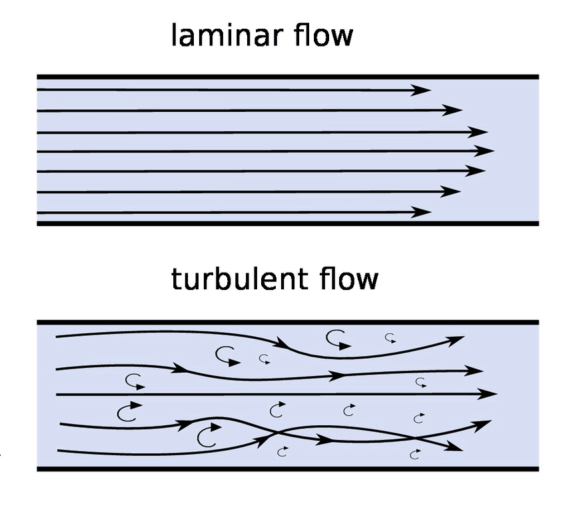
\includegraphics[width=0.4\textwidth, height=.55\textheight]{./Ressourcen/Praesentation/Bilder/laminar_turbulent.png}

\end{multicols}
\vspace*{-4mm}
Taken from \url{https://diffzi.com/laminar-flow-vs-turbulent-flow/}
\end{frame}
\clearpage

\begin{frame}
    \frametitle{Background -- RANS}
	\vspace*{8mm}
	\textbf{Reynolds number $Re$}:

\begin{PraesentationAufzaehlung}
		\item dimensionless constant
		\item needed for calculation of turbulence models
		\item magnitude decides flow (laminar, turbulent)
		\item  affects lift and drag coeffcients
\end{PraesentationAufzaehlung}

\end{frame}
\clearpage

\begin{frame}
    \frametitle{Background -- Reynolds number: $<1$}
	\vspace*{8mm}
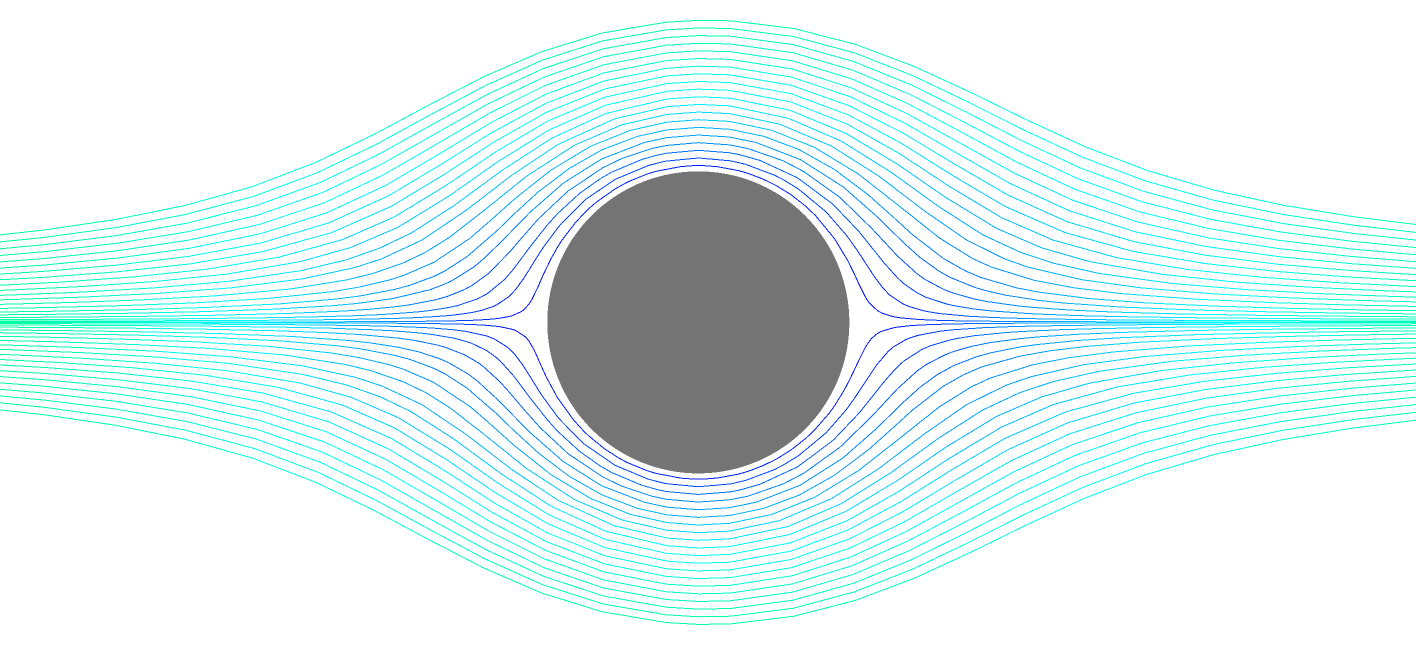
\includegraphics[width=0.8\textwidth, height=.55\textheight]{./Ressourcen/Praesentation/Bilder/Re/re_1.png}

Taken from \url{https://www.computationalfluiddynamics.com.au/reynolds-number-cfd/}
\end{frame}
\clearpage

\begin{frame}
    \frametitle{Background -- Reynolds number: $\approx 10$}
	\vspace*{8mm}
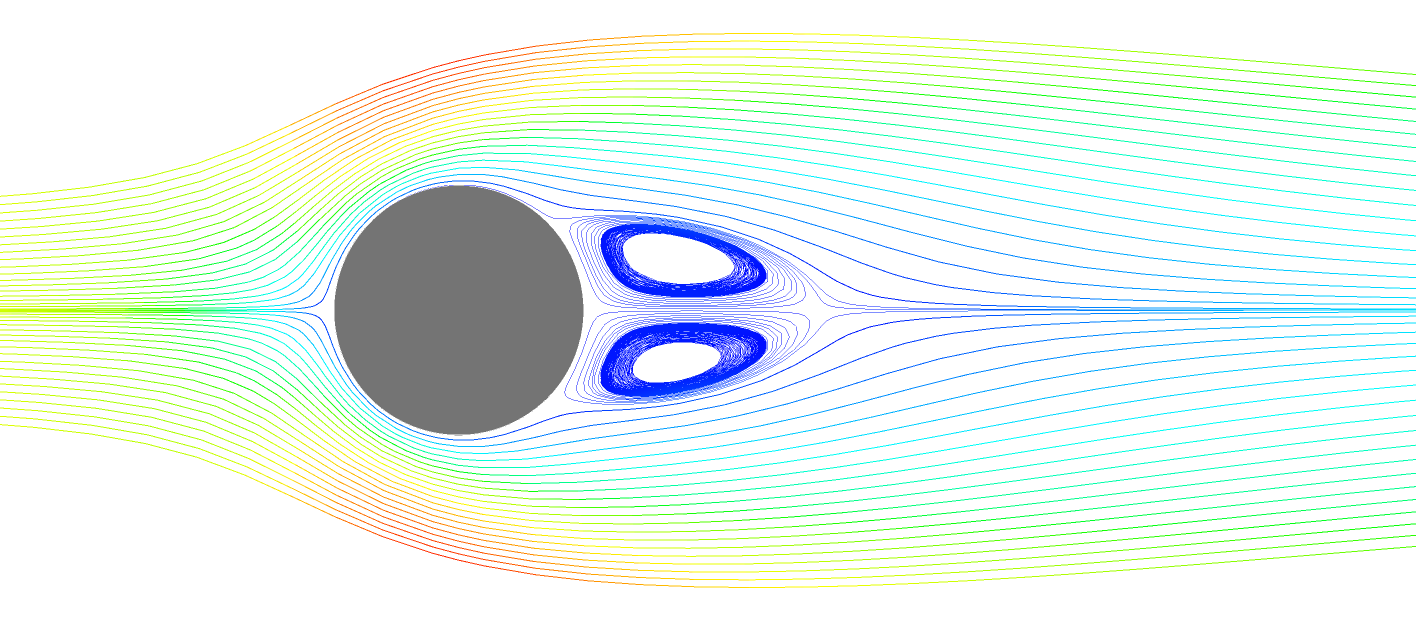
\includegraphics[width=0.8\textwidth, height=.55\textheight]{./Ressourcen/Praesentation/Bilder/Re/re_10.png}

Taken from \url{https://www.computationalfluiddynamics.com.au/reynolds-number-cfd/}
\end{frame}
\clearpage

\begin{frame}
    \frametitle{Background -- Reynolds number: $\approx 1 \cdot 10^5$}
	\vspace*{8mm}
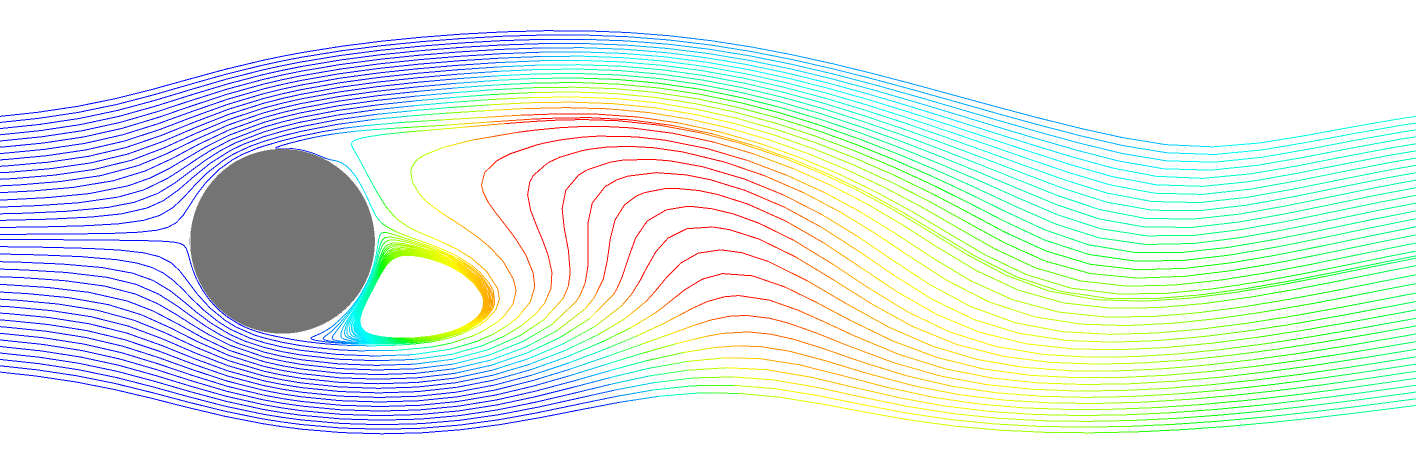
\includegraphics[width=0.8\textwidth, height=.55\textheight]{./Ressourcen/Praesentation/Bilder/Re/re_1e5.png}

Taken from \url{https://www.computationalfluiddynamics.com.au/reynolds-number-cfd/}
\end{frame}
\clearpage

%%%%%%%%%%%%%%%%%%%%%%%%%%
%% Folie: Background    %%
%%%%%%%%%%%%%%%%%%%%%%%%%%
\begin{frame}
    \frametitle{Background -- Convolutions}
\vspace*{5mm}
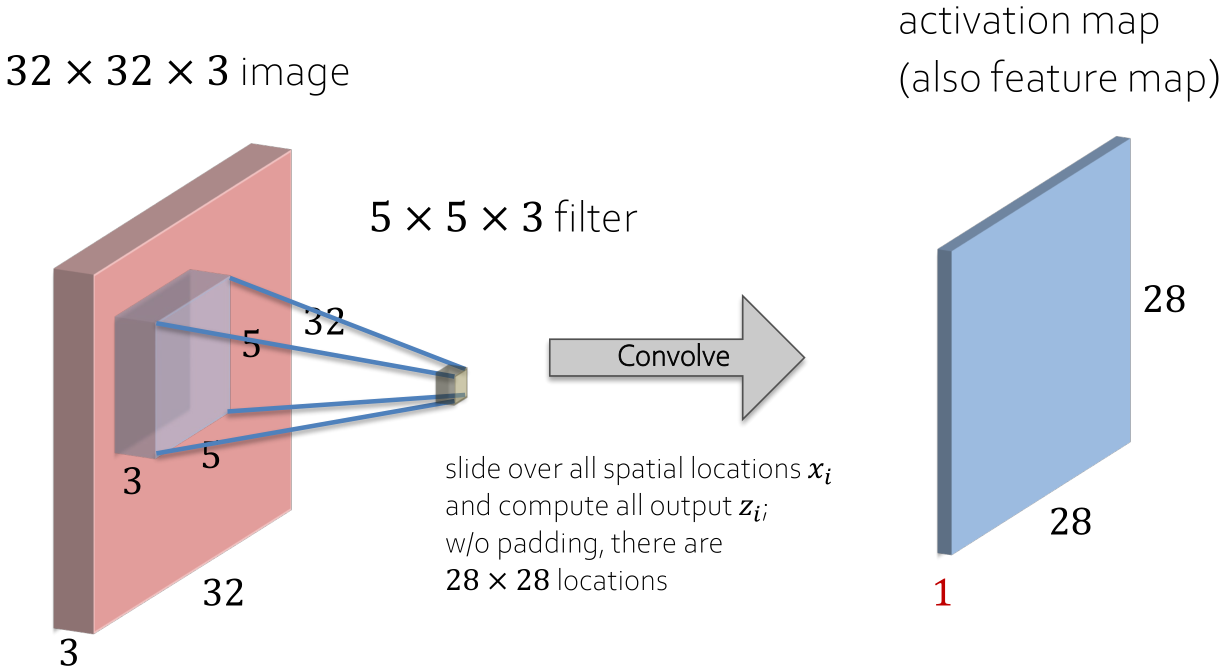
\includegraphics[width=0.8\textwidth, height=.55\textheight]{./Ressourcen/Praesentation/Bilder/conv_bsp.png}%

Taken from I2DL WS19/20 (TUM)
    
\end{frame}
\clearpage

%%%%%%%%%%%%%%%%%%%%%%%%%%
%% Folie: Background    %%
%%%%%%%%%%%%%%%%%%%%%%%%%%
\begin{frame}
    \frametitle{Background -- Convolutions}

Low-Level Features, Mid-Level Features, High-Level Features: each filter captures different characteristics

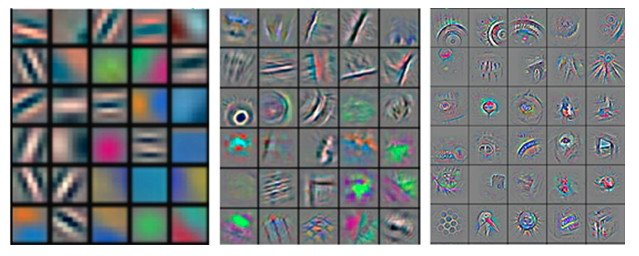
\includegraphics[width=0.8\textwidth, height=.55\textheight]{./Ressourcen/Praesentation/Bilder/features.png}%
\vspace*{-5mm}

Taken from \url{https://arxiv.org/pdf/1311.2901.pdf}   
    
\end{frame}
\clearpage